%!TEX root = ../main-anran-ma.tex 
% so I can build in this tex file too. 
%************************************************
% \setcounter{theorem}{6}
\chapter{A Proof System}\label{ch:system} % $\mathbb{ZNR}$
%************************************************

% \section{Literature Review}

% Here is a description of all the triples. 
% \todo{Literature review section}



We are interested in studying the \define{necessary liberal precondition}, a weakening of the weakest liberal precondition: 
$$wlp.C.F\implies G$$
The weaker $G$ can contain various preconditions: on the one hand, $G$ can be so general that it is satisfied by any program state; on the other hand, a $G$ that is barely weaker than $wlp.C.F$ is also not much different from the latter. 
Alternatively, $G$ can also contain all kinds of preconditions that starting from it, any postcondition is reachable. 
One thing we are certain about, though, is that a program with an original state satisfying $\neg G$ will terminate, and the final state can satisfy $\neg F$: 
\begin{align*}
wlp.C.F\implies G & = \neg G \implies \neg wlp.C.F \\
	& = \neg G \implies wp.C.\neg F 
	\hspace{0.3\textwidth} \mid {\thm{conjugate}}
\end{align*}
In the upcoming sections, we first discuss various forms that the necessary liberal precondition can take and try to identify a $G$ that is most characteristic. 
We proceed then to propose a proof system stemming from the necessary liberal precondition and show its usefulness using an example. \todo{rewrite}

\section{Preconditions and Postconditions}
\subsection{wp and Related}
\begin{figure}[ht!]\centering
	\subfloat[Weakest precondition (angelic non-determinism)\label{subfig:wpa}]{
		\includesvg[width=0.4\textwidth]{image/wpa.svg}}
	\hfill
	\subfloat[Weakest precondition (demonic non-determinism)\label{subfig:wpd}]{
		\includesvg[width=0.4\textwidth]{image/wpd.svg}}

	\subfloat[Weakest liberal precondition (angelic non-determinism)\label{subfig:wlpa}]{
		\includesvg[width=0.4\textwidth]{image/wlpa.svg}}
	\hfill
	\subfloat[Weakest liberal precondition (demonic non-determinism)\label{subfig:wlpd}]{
		\includesvg[width=0.4\textwidth]{image/wlpd.svg}}
	\caption{wp, wlp with Angelic and Demonic Non-determinism}
	\label{fig:wp-family}
\end{figure}
\autoref{fig:wp-family} shows the impact of the interpretation of non-determinism on the semantics of the wp and wlp transformers. 
The subscripts $_a$ and $_d$ correspond to angelic and demonic, respectively. 

With angelic non-determinism, we consider the non-deterministic choice to resolve in our favor, which means that if one of the possible paths from this non-deterministic choice can lead to the desired postcondition, we regard the precondition as a valid precondition. 
Graphically, the green arrows in \autoref{subfig:wpa} and \autoref{subfig:wlpa} are included in the weakest (liberal) precondition when we regard the non-determinism as angelic. 
Formally, the decision to look at the non-deterministic choice as angelic is reflected by the use of disjoints in its definition, for example, 
$$wp.C.(\{C_1\}\square \{C_2\}) = wp.C_1.F\vee wp.C_2.F$$ in \autoref{tab:wp-wlp}.

On the other hand, if the non-deterministic choice is regarded as demonic, we are pessimistic over the result of the non-deterministic choice: we think it will not resolve in our favor, hence we are only confident to include a condition into the valid precondition set, if all possible paths end satisfying our desired postcondition upon termination. 
Graphically, the green arrows are not included in $wp$ and $wlp$ in \autoref{subfig:wpd} and \autoref{subfig:wlpd}. 
The definition is then using conjuncts instead of disjuncts, like 
$$wlp.C.(\{C_1\}\square \{C_2\}) = wlp.C_1.F\wedge wlp.C_2.F$$  in \autoref{tab:wp-wlp}.

The choice is somewhat artificial, depending on what properties the author wishes for their transformers.
For example, Dijkstra and Scholten choose demonic non-determinism for wp and wlp transformers, acquiring a property by definition~\cite{dijkstra90}: 
$$wp_d.C.F = wlp_d.C.F \wedge wp_d.C.true $$
meaning that by finding the weakest liberal precondition and proving termination, one conveniently finds the weakest precondition of the same program and postcondition. 
Graphically, one needs only to re-place the dashed arrows indicating non-termination to get from \autoref{subfig:wpa} to \autoref{subfig:wlpa} and vice versa, or from  \autoref{subfig:wpd} to \autoref{subfig:wlpd} and vice versa. 

This is especially useful when trying to underapproximate the weakest precondition, %TODO: add reference?
or in other words, finding valid Hoare Triple, considering that \hoare{G}{C}{F} is a valid Hoare Triple (with regard to total correctness, meaning that we supplement the original axioms~\cite{hoare69} with rules to prove termination~\cite{manna74}) if and only if $G\implies wp.C.F$.
% The rule also applies if one chooses both angelic 

Conversely, if one were to choose different views on non-determinism with wp and wlp transformers, we end up with a different property that wp and wlp are each other's conjugates~\cite{dijkstra76,zhang22}: 
$$ wp_a.C.F = \neg wlp_d.C.\neg F $$ 
this indicates a duality between $wp_a$ and $wlp_d$ in the sense that by defining one transformer, we can arrive at the other by negation. 
Graphically, we can ``flip'' \autoref{subfig:wpd} to arrive at \autoref{subfig:wlpa} and vice versa, or ``flip'' \autoref{subfig:wpa} to arrive at \autoref{subfig:wlpd} and vice versa, like in \autoref{fig:flip-wp-wlp}. 
\begin{figure}[ht]
	\centering
	\includesvg[width=.9\linewidth]{image/flip-wp-wlp.svg}
	\caption{wp$_a$ and wlp$_d$ Are Conjugates}
	\label{fig:flip-wp-wlp}
\end{figure}

These relations can be summed up as in \autoref{fig:wp-family-relation}. 
The choice whether to resolve the non-determinism angelically or demonically for wp and wlp depends then on which of the relations the author prefers. 
\begin{figure}[ht]
	\centering
	\includesvg[width=.5\linewidth]{image/wp-family-relation.svg}
	\caption{Relations in wp-Family}
	\label{fig:wp-family-relation}
\end{figure}

In this thesis, we prefer wp with angelic non-determinism and wlp with demonic non-determinism, because this choice gifts us Galois connection between the precondition transformers and the postcondition transformers~\cite{zhang22}, which we will illustrate in the next section: 
\begin{theorem}{thm:galois-wp}[Galois connection between wp and slp]
	$$wp_a.C.F \implies G \text{ if and only if }F\implies slp_d.C.G$$
\end{theorem}

\begin{theorem}{thm:galois-wlp}[Galois connection between wlp and sp]
	$$G \implies wlp_d.C.F \text{ if and only if } sp_a.C.G\implies F$$
\end{theorem}

\subsection{sp and Related}
The strongest postcondition was originally discussed as a side-product of the wp and wlp transformers by Dijkstra and Scholten~\cite{dijkstra90}. 
$sp.S.Y$ is meant to describe ``those final states for which there exists a computation under control of S that belongs to the class \textit{initially Y}'', but it has found more important utilities. 
For example, de Vries and Koutavas~\cite{vries11} use sp to reason with randomized algorithms, although they called it \define{weakest postconditions}. 
O'Hearn~\cite{ohearn2020IncorrectnessLogic} uses sp to define \define{incorrectness logic} by underapproximating it, building the theoretical foundation to a new method of identifying errors in programs. 

Instead of questioning about termination and final states upon termination, like the precondition transformers, the postcondition transformers question about reachability and initial states that can reach the desired postconditions. 
The choice of angelic and demonic non-determinism also plays a rule while determining the semantics of the postcondition transformers, as shown in \autoref{fig:sp-family}. 

\begin{figure}[ht!]\centering
	\subfloat[Strongest postcondition (angelic non-determinism)\label{subfig:spa}]{
		\includesvg[width=0.4\textwidth]{image/spa.svg}}
	\hfill
	\subfloat[Strongest postcondition (demonic non-determinism)\label{subfig:spd}]{
		\includesvg[width=0.4\textwidth]{image/spd.svg}}

	\subfloat[Strongest liberal postcondition (angelic non-determinism)\label{subfig:slpa}]{
		\includesvg[width=0.4\textwidth]{image/slpa.svg}}
	\hfill
	\subfloat[Strongest liberal postcondition (demonic non-determinism)\label{subfig:slpd}]{
		\includesvg[width=0.4\textwidth]{image/slpd.svg}}
	\caption{sp, slp with Angelic and Demonic Non-determinism}
	\label{fig:sp-family}
\end{figure}

Note that while sp is well-researched, slp is less investigated to the best of our knowledge. 
For example, Wulandari and Plump~\cite{wulandari2020VerifyingGraphPrograms} defined and proved soundness for slp, but only for loop-free programs. 
While Li et al.~\cite{li2011NonlinearMathematicsUncertainty} proposed the definition of slp including loops, but did not include proof for soundness and completeness. 
Even so, the semantics of slp is rather undisputed: slp should be sp joint with all unreachable postconditions. 

Following the same principles as the ones for precondition transformers, we can deduce a similar relation between the postcondition transformers with different resolution for non-determinism, as seen in \autoref{fig:sp-family-relation}. 
The main difference is that the arrows pointing up are not labelled with termination, but reachability. 

\begin{figure}[ht]
	\centering
	\includesvg[width=.5\linewidth]{image/sp-family-relation.svg}
	\caption{Relations in sp-Family}
	\label{fig:sp-family-relation}
\end{figure}

Supplementing the Galois connection specified in \thm{thm:galois-wp} and \thm{thm:galois-wlp}, we arrive at \autoref{fig:wp-sp-relation}. 
It is now obvious that we chose to resolve non-determinism exactly like the colored ones in \autoref{fig:wp-sp-relation}, so that we can conveniently connect the pre- and postcondition transformers. 

\begin{figure}[ht]
	\centering
	\includesvg[width=.5\linewidth]{image/wp-sp-relation.svg}
	\caption{Connecting wp-Family and sp-Family}
	\label{fig:wp-sp-relation}
\end{figure}

\section{A Precondition Weaker Than the Weakest Liberal Precondition}
In \autoref{sec:wlp} we define the weakest liberal precondition and state that it characterizes all the preconditions under whose control the program either \imptt{diverges} or \imptt{will} terminate in a state satisfying $F$. 
We are certain to use ``will'' instead of ``can'', the non-deterministic choice is viewed as demonic, so the behavior of wlp can be depicted by \autoref{subfig:wlpd}. 
We can categorize the executions of the program in four ways: 
\begin{enumerate}
	\item the dashed arrow means non-terminating executions; 
	\item the black arrows are executions starting from an initial state satisfying $wlp.C.F$ and only terminating in final states satisfying $F$; 
	\item the green arrows are the executions starting from an initial state satisfying $\neg wlp.C.F$ but can terminate in states either satisfying $F$ or satisfying $\neg F$;
	\item the red arrow represents executions starting from an initial state satisfying $\neg wlp.C.F$ and only terminating in final states satisfying $\neg F$. 
\end{enumerate}


\begin{figure}[ht!]\centering
	\subfloat[Weakest liberal precondition (demonic non-determinism)\label{subfig:wlpd}]{
		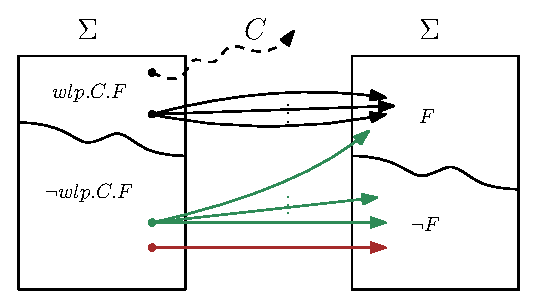
\includegraphics[width=0.4\textwidth]{image/wlp-g/wlpd.eps}}
	\hfill

	\subfloat[Precondition $G$ with $wlp.C.F\implies G$ and $G$ contains some green arrows\label{subfig:wlp-g-g}]{
		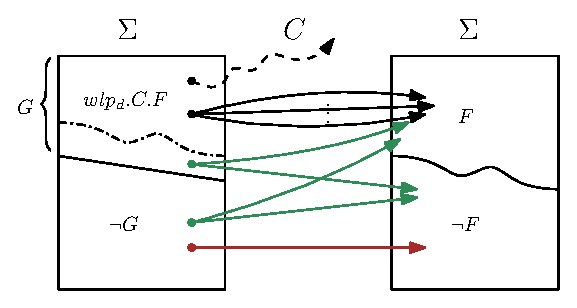
\includegraphics[width=0.45\textwidth]{image/wlp-g/wlp-g-g.eps}
	}
	\hfill
	\subfloat[Precondition $G$ with $wlp.C.F\implies G$ and $G$ contains all the green arrows\label{subfig:wlp-g-gg}]{
		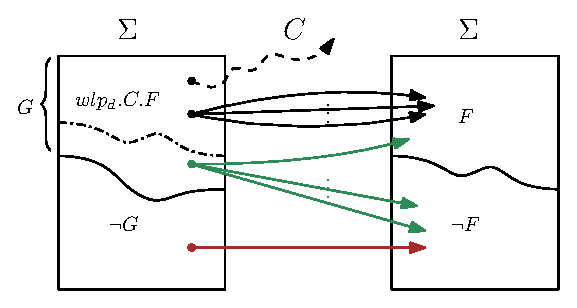
\includegraphics[width=0.45\textwidth]{image/wlp-g/wlp-g-gg.eps}
	}

	\subfloat[Precondition $G$ with $wlp.C.F\implies G$ and $G$ contains some red arrows\label{subfig:wlp-g-r}]{
		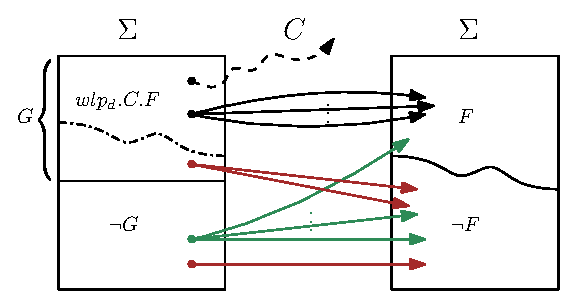
\includegraphics[width=0.45\textwidth]{image/wlp-g/wlp-g-r.eps}
	}
	\hfill
	\subfloat[Precondition $G$ with $wlp.C.F\implies G$ and $G$ contains all the red arrows\label{subfig:wlp-g-rr}]{
		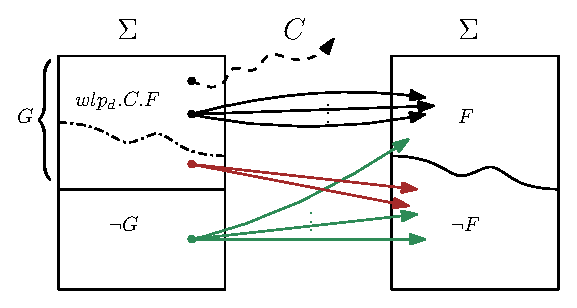
\includegraphics[width=0.45\textwidth]{image/wlp-g/wlp-g-rr.eps}
	}
\caption{Case Distinction of Preconditions Weaker Than wlp}
\label{fig:wlp-g-1}
\end{figure}

\begin{figure}[ht!]\centering
	\ContinuedFloat
	\subfloat[Precondition $G$ with $wlp.C.F\implies G$ and $G$ contains some green arrows and some red arrows\label{subfig:wlp-g-gr}]{
		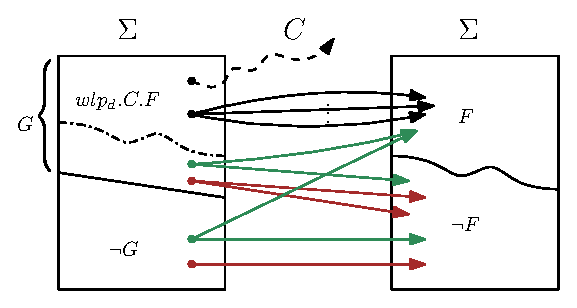
\includegraphics[width=0.45\textwidth]{image/wlp-g/wlp-g-gr.eps}
	}
	\hfill
	\subfloat[Precondition $G$ with $wlp.C.F\implies G$ and $G$ contains all the green arrows and some red arrows\label{subfig:wlp-g-ggr}]{
		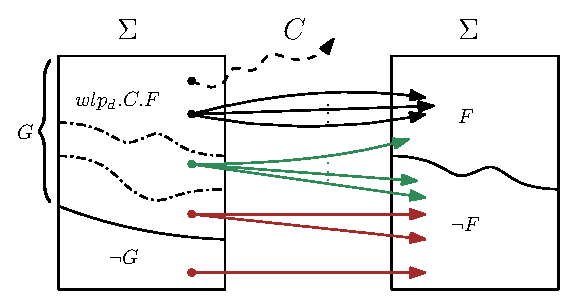
\includegraphics[width=0.45\textwidth]{image/wlp-g/wlp-g-ggr.eps}
	}

	\subfloat[Precondition $G$ with $wlp.C.F\implies G$ and $G$ contains some green arrows and all the red arrows\label{subfig:wlp-g-grr}]{
		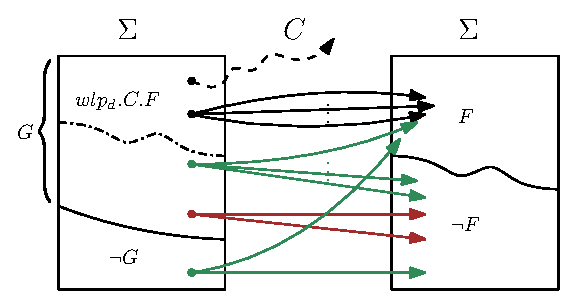
\includegraphics[width=0.45\textwidth]{image/wlp-g/wlp-g-grr.eps}
	}
	\hfill
	\subfloat[Precondition $G$ with $wlp.C.F\implies G$ and $G$ contains all the arrows\label{subfig:wlp-g-ggrr}]{
		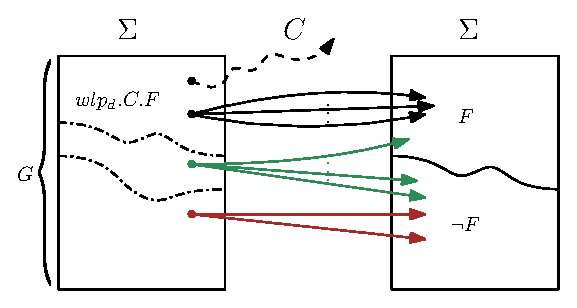
\includegraphics[width=0.45\textwidth]{image/wlp-g/wlp-g-ggrr.eps}
	}
\caption{Case Distinction of Preconditions Weaker Than wlp (Cont.) }
\label{fig:wlp-g-2}
\end{figure}
If we were to weaken the precondition, it can happen in various ways as shown in \autoref{subfig:wlp-g-g}{\color{RoyalBlue}-9}. 
However, $G$ spikes our interest when it takes the form as in \autoref{subfig:wlp-g-gg}, because under its control, the program always \imptt{can} reach a final state satisfying $F$ if it terminates, while with an initial state satisfying $\neg G$, the program is \imptt{will} terminate satisfying $\neg F$. 
This behavior is exactly the behavior of wlp, if we were to regard the non-deterministic choice as angelic, as hinted by the similarities between \autoref{subfig:wlp-g-gg} and \autoref{subfig:wp-angelic}. 
We thus first investigate this special case, before proceeding with $G$ in general. 

\subsection{A Special Case} %: $G$ is wlp with Angelic Non-determinism
Dual to the semantics of wp and wlp as shown in \thm{wp-sound} and \thm{wlp-sound}, we can deduce the semantics of wlp with angelic non-determinism (denoted by \define{wlp$_a$}) recalling the representation for non-termination mentioned in \autoref{sec:big-step}: 
\begin{statement}{wlpa-sound}[Semantics of $wlp_a$]
\ \vspace{-1.5mm}
\[
wlp_a.C.F = \{ \sigma\in\S \mid
\neg(\exists \tau\in\S: \sigma\goto{C}\tau) \ \ \vee\ \ 
(\exists \tau\in\S: \sigma\goto{C}\tau\wedge  \tau\vDash F)
 \}
\]
% \label{thm:wlpa}
\end{statement}

Luckily, we can find statements using wlp and sp that captures this specific $G$, hence giving us a way to express wlp$_a$ without having to define it: 
\begin{lemma}{wlpa-g}[Angelic wlp implies G]
\ \\ \vspace{-3mm}
	\[\hspace{-2mm}
	\text{ if \ \ \ \ } 
	(wlp.C.F\implies G)
	\ \wedge\ 
	(sp.C.\neg G \implies \neg F) 
	\text{\ \ \ \  then\ \ \ \  } 
	wlp_a.C.F \implies G
	\] 
	\label{lem:wlp-g}
\end{lemma}
The second prerequisite \mathl{sp.C.\neg G \implies \neg F } states that from $\neg G$ we are only allowed to reach $\neg F$, making sure that all green arrows as in \autoref{fig:wlp-g-1} are included in $G$. 

% macros for referencing to lines in this chapter
\newcommand{\lblth}[1]{\hypertarget{3.#1}{{\text{#1}}}}
\newcommand{\refth}[1]{\hyperlink{3.#1}{{\text{Line (#1)}}}}
\begin{proof}
	The assumption expresses that for any state $\sigma\in\S$:
\begin{align*} 
	wlp.C.F\implies G\  \Leftrightarrow&\ \sigma\in wlp.C.F \implies \sigma\in G \\
	\Leftrightarrow&\ ( \forall \tau\in\S:\ \sigma\goto{C}\tau\implies  \tau\in F) \implies \sigma\in G \tag*{$\mid$ \thm{wlp-sound}} \\
	\Leftrightarrow&\ (\forall \tau\in\S:\ \neg(\sigma\goto{C}\tau)\ \vee\ \tau\in F) \implies \sigma\in G \\
	\Leftrightarrow&\ \neg(\exists\tau\in\S:(\sigma\goto{C}\tau)\ \wedge\ \neg(\tau\in F)) \implies \sigma\in G \tag{\lblth{a}} \\
	% && \mid \lblth{a} \\
	% &\ \ \ \  \vee (\forall \tau.\sigma\goto{C}\tau:\tau\in F \Longrightarrow \sigma\in G) 
		% \hspace{0.017\textwidth} \mid \lblth{b} \\
	%
\end{align*}
Also, for any state $\tau\in\S$: 
\begin{align*}
	sp.C.\neg G \implies \neg F \Leftrightarrow&\ \tau\in sp.C.\neg G \implies \tau\in \neg F \\
	\Leftrightarrow&\  (\exists \mu\in\S:\ \mu\goto{C}\tau\ \wedge\ \mu\in\neg G )\implies \tau\in\neg F \tag*{$\mid$ \thm{sp-sound}}\\
	% &\hspace{0.45\textwidth} \mid \thm{sp-sound}\\
	\Leftrightarrow&\  \neg (\tau\in\neg F) \implies \neg (\exists \mu\in\S:\ \mu\goto{C}\tau\ \wedge\ \mu\in\neg G ) \\
	\Leftrightarrow&\  \tau\in F \implies \forall \mu\in\S:\ \neg (\mu\goto{C}\tau\ \wedge\ \mu\in\neg G)\\
	\Leftrightarrow&\  \tau\in F \implies \forall \mu\in\S:\ \neg (\mu\goto{C}\tau)\ \vee\ \neg(\mu\in\neg G)\\
	\Leftrightarrow&\  \tau\in F \implies \forall \mu\in\S:\ \neg (\mu\goto{C}\tau)\ \vee\ \mu\in G
	\tag{\lblth{b}} \\
	%
\end{align*}
Our goal is to prove that for any state $\sigma\in\S$:
\begin{align*}
	wlp_a.C.F \implies G \Leftrightarrow&\ \sigma\in wlp_a.C.F \implies \sigma\in G \\
	\Leftrightarrow&\  \neg(\exists \tau\in\S: \sigma\goto{C}\tau) \ \vee\ 
	(\exists \tau\in\S: \sigma\goto{C}\tau\wedge  \tau\in F)\\
	&\ \ \ \ \implies \sigma\in G \tag*{$\mid$ \stm{wlpa-sound}}\\
	% &\hspace{0.45\textwidth} \mid \stm{wlpa-sound}\\
	\Leftrightarrow&\  (\neg(\exists \tau\in\S: \sigma\goto{C}\tau)\implies \sigma\in G ) \tag{\lblth{c}}\\
	% && \mid \lblth{c}\\
	&\ \wedge\ ((\exists \tau\in\S: \sigma\goto{C}\tau\wedge  \tau\in F)\implies\sigma\in G) \tag{\lblth{d}}\\
	% && \mid \lblth{d}
\end{align*}
We can prove \lem{wlpa-g} by proving that \refth{a} implies \refth{c} and that \refth{b} implies \refth{d}.
For any state $\sigma\in\S$, we first prove (a)$\implies$(c):
\begin{align*}
	% \text{(a)}\implies\text{(c)}:\text{ for any } \\
	true 
	\Leftrightarrow&\ (\exists\tau\in\S:(\sigma\goto{C}\tau)\ \wedge\ \neg(\tau\in F)) \implies (\exists\tau\in\S:\sigma\goto{C}\tau)\\ 
	\Leftrightarrow&\ \neg(\exists\tau\in\S:\sigma\goto{C}\tau) \implies \neg(\exists\tau\in\S:(\sigma\goto{C}\tau)\ \wedge\ \neg(\tau\in F))  \\ 
	\Rightarrow&\ \neg(\exists\tau\in\S:\sigma\goto{C}\tau) \implies \sigma\in G \tag*{$\mid$ \refth{a}}\\
\end{align*}
It is also valid that for any state $\sigma\in\S$, (b)$\implies$(d). 
Assume there exists $\tau\in\S$ such that for some state $\sigma\in\S$, 
$$\sigma\goto{C}\tau\ \wedge\  \tau\in F \text{ is valid. }$$
Then we conclude from \refth{b} that 
$$\forall \mu\in\S:\ \neg (\mu\goto{C}\tau)\ \vee\ \mu\in G$$
Since $\sigma\in\S$, it follows that $\neg(\sigma\goto{C}\tau)\ \vee\ \sigma\in G$. 
We already know that $\sigma\goto{C}\tau$, hence $\sigma\in G$ must be true, therefore proving \refth{d}. 
\end{proof}


\begin{lemma}{g-wlpa}[G implies angelic wlp]
\ \\ \vspace{-3mm}
	\[%\hspace{-5mm}
	\text{ if \ \ \ \ } 
	(P{\implies} G) \implies \neg(sp.C.P {\implies} \neg F)
	\text{\ \ \ \  then\ \ \ \  } 
	G {\implies} wlp_a.C.F
	\] 
\end{lemma}
Here, the prerequisite states that we do not allow executions starting from $G$ that \imptt{only} finish in $\neg F$, making sure that $G$ does not include the red arrows as in \autoref{fig:wlp-g-1}.  

\begin{proof}
	The assumption expresses that for any state $\sigma\in\S$:
\begin{align*} 
	&\ P\implies G \implies \neg(sp.C.P \implies \neg F) \\ 
	\Leftrightarrow&\ P\implies G \implies \neg(\forall\tau\in\S:\tau\in sp.C.P{\implies}\tau\in\neg F) \\ 
	\Leftrightarrow&\ P\implies G \implies \exists\tau\in\S:\neg(\tau\in sp.C.P{\implies}\tau\in\neg F) \\ 
	\Leftrightarrow&\ P\implies G \implies \exists\tau\in\S:\tau\in sp.C.P\ \wedge\ \neg(\tau\in\neg F) \\ 
	\Leftrightarrow&\ P\implies G \implies \exists\tau\in\S:\tau\in sp.C.P\ \wedge\ \tau\in F \\ 
	\Leftrightarrow&\ P\implies G \implies \exists\tau\in\S:(\exists \mu\in\S:\ \mu\goto{C}\tau\ \wedge\ \mu\in P)\ \wedge\ \tau\in F \tag*{$\mid$ \thm{sp-sound}}\\ 
	\Leftrightarrow&\ \sigma\in P {\implies} \sigma\in G {\implies} \exists\tau\in\S:(\exists \mu\in\S:\ \mu\goto{C}\tau\ \wedge\ \mu\in P)\ \wedge\ \tau\in F \tag{\lblth{e}}\\ 
	%
\end{align*}
Our goal is to prove that for any state $\sigma\in\S$:
\begin{align*}
	&\ G\implies wlp_a.C.F \\ 
	\Leftrightarrow&\  \sigma\in G\implies\sigma\in wlp_a.C.F\\
	\Leftrightarrow&\ \sigma\in G\implies \neg(\exists \tau\in\S: \sigma\goto{C}\tau) \ \vee\ 
	(\exists \tau\in\S: \sigma\goto{C}\tau\wedge  \tau\in F) \tag*{$\mid$ \stm{wlpa-sound}}\\
\end{align*}
For some state $\sigma\in\S$, assume $\sigma\in G$, then we can construct set $P=\{\sigma\}$ such that the prerequisites in \refth{e} holds. 
Consequently, the postrequisite in holds. 
Now we can find witnesses $\mu$ and $\tau$ such that
$$
\mu\goto{C}\tau\ \wedge\ \mu\in P\ \wedge\ \tau\in F 
$$
Since $P$ is a singleton set, $\mu$ can only be $\sigma$. 
Then we have found a witness $\tau$ such that $\sigma\goto{C}\tau$ and $\tau\in F$, satisfying the postrequisite of our goal. 
\end{proof}

\begin{corollary}{g=wlp}[G equivalent to angelic wlp]
% \begin{align*}
	\ \\
	$\text{ if } \ wlp.C.F{\implies} G \ \wedge\ 
	sp.C.\neg G {\implies} \neg F 
	\ \text{ and } \ 
	P{\implies} G \implies \neg(sp.C.P {\implies} \neg F) \\
	\text{ then }\ G = wlp_a.C.F$
% \end{align*}	
\end{corollary}

\subsection{The General Case}
While having restrictions on $G$ yields interesting results, without the restrictions we can still find useful characteristics. 
As shown in \autoref{fig:wlp-g-2}, $G$ can contain all possible initial states, which can be the starting points of black, green, red, or dashed arrows, representing executions terminating in states satisfying $F$, $F$ or $\neg F$, $\neg F$, or non-terminating, respectively. 
As a result, we can not make much statements without adding extra restrictions to $G$. 
However, we can see from \autoref{fig:wlp-g-2} that $\neg G$ does not contain any \imptt{black} or \imptt{dashed} arrows in all cases. 
In other words, if program $C$ starts in any initial state satisfying $\neg G$, then either $G$ is empty, or
\begin{itemize}
	\item its executions terminate, and
	\item there exists an execution that ends up in a final state that satisfies $\neg F$. 
\end{itemize}

This corresponds to the semantics of the wp transformer as shown in \thm{wp-sound}, hinting that \hoare{\neg G}{C}{\neg F} is a valid Hoare triple. 
The question then naturally arises: why do we concern ourselves with $G$, if we can just prove our specifications using wp or Hoare triples? 
To demonstrate the answer, we analyze the example written in \autoref{lst:pererson}. 

\begin{lstlisting}[caption={Thread $A$ Hoping to Access Critical Section}, label={lst:pererson}, language=java, numbers=left, stepnumber=1, captionpos=b,escapechar=|,frame=single]
	... // leave non-critical section
	turn := B; |\label{line:p-2}|
	while (turn != A) do 
		turn := A |$\square$| turn := B |\label{line:p-4}|
		// modeling the behavior of other threads
	critA := true;|\label{line:p-6}|
	... // enter critical section  
\end{lstlisting}

The pseudocode is modified from Peterson's mutual exclusion algorithm~\cite{peterson1981}, but we are now only concerned with one of possibly many threads.
Our thread $A$ is trying to enter some critical section but only have limited knowledge as to what other threads might also want to access the same critical section: $A$ is only aware of thread $B$ that also wants to enter critical section. 

To have a \imptt{fair} system, thread $A$ gives $B$ the turn after leaving non-critical section as written in \moreref{line}{line:p-2} of \autoref{lst:pererson}. 
Otherwise, thread $A$ might never enter the while-loop and directly skip ahead to \moreref{line}{line:p-6} to enter the critical section, without giving other threads a chance. 
\moreref{Line}{line:p-4} models the behavior of other threads in the system: while $A$ is waiting for its turn, thread $B$ might also have just left the non-critical section and gave the turn to $A$; or some other thread than $A$ or $B$ might have given the turn to $B$.~\footnote{We will see with the calculation for wlp of this while-loop that it makes no difference whether we include more non-deterministic choices like $turn := C\ \square\ turn := D\ \square\ \dots$.} 

Mutual exclusion requires that no threads are simultaneously in the critical section. 
In this case, a state we definitely want to avoid is where the values of $critA$ and $critB$ are both true. 
In other words, the postcondition 
$$F=\{\sigma\in\S\mid \sigma.critB=true\}$$ 
after \moreref{line}{line:p-6} in \autoref{lst:pererson} is an undesirable postcondition.

Filling in this $F$ after \moreref{line}{line:p-6} and calculating the weakest liberal precondition backwards according to \autoref{tab:wp-wlp}, we arrive at the conditions as shown in \autoref{lst:critB}. 
For better readability, we shorten predicates like $F$ to $\{critB\}$.

\begin{lstlisting}[caption={Weakest Liberal Precondition w.r.t Postcondition $F=\{\sigma\in\S\mid \sigma.critB=true\}$ }, label={lst:critB}, language=java, numbers=left, stepnumber=1, captionpos=b,escapechar=|,frame=single]
	... // leave non-critical section
	|\imptt{\{critB\}}|
	turn := B;
	|\imptt{\{critB\}}\label{line:c-4}|
	while (turn != A) do 
		turn := A |$\square$| turn := B 
		// modeling the behavior of other threads
	|\imptt{\{critB\}}\label{line:c-8}|
	critA := true;
	|\imptt{\{critB\}}|
	... // enter critical section  
\end{lstlisting}

The only non-obvious step in \autoref{lst:critB} is from \moreref{line}{line:c-8} to \moreref{line}{line:c-4}. 
Remember from \autoref{tab:wp-wlp} that the wlp for while-loops is defined with the greatest fixed point operator: 
\[
	wlp.(\text{while }(\varphi)\ \{C'\}).F = gfp\ X.\ (\neg\varphi\wedge F)\vee(\varphi\wedge wlp.C'.X)
\]
We can simply follow the iteration to find the greatest fixed point of a function until we see a pattern, then prove by natural induction that the solution we found is indeed the greatest fixed point (see \thm{gfp}).

\begin{lemma}{critB}
	$wlp.WHILE.\{critB\} = \{critB\}$
	where $WHILE := while\ (\varphi)\ do\ C'$, $\varphi := \{turn!=A\}$,\ \ and $C':=(turn:=A\ \square\ turn:=B)$. 
\end{lemma}
\begin{proof} 
	\begin{align*}
		\text{Let }\Phi(X) :=&\ \neg\varphi\wedge F\ \ \vee\ \ \varphi\wedge wlp.C'.X\\ 
		=&\ \{turn=A\}\wedge \{critB\}\ \ \vee\ \ \{turn!=A\} \wedge wlp.C'.X\\
		\text{Then }\Phi(true) =&\ \{turn=A\}\wedge \{critB\}\ \ \vee\ \ \{turn!=A\} \wedge wlp.C'.true \\ 
		\overset{\thm{wlp-true}}{=}&\ \{turn=A\}\wedge \{critB\}\ \ \vee\ \ \{turn!=A\} \wedge true \\
		% &\hspace{0.45\textwidth} | \ \thm{wlp-true} \\
		=&\ \{turn != A\} \vee \{critB\} \\
	\end{align*}
	\begin{align*}
		\text{Also, } wlp.C'.\Phi(True)=&\ wlp.(turn:=A\ \square\ turn:=B).\Phi(true)\\
		\overset{\autoref{tab:wp-wlp}}{=}&\ wlp.(turn:=A).(\{turn != A\} \vee \{critB\}) \\
		&\ \wedge wlp.(turn:=B).(\{turn != A\} \vee \{critB\})\\
		\overset{\autoref{tab:wp-wlp}}{=}&\ (\{A!=A\}\vee\{critB\})\wedge\{B!=A\}\vee\{critB\}\\
		=&\ \{critB\}\wedge true \\
		=&\ \{critB\}
	\end{align*}
	\begin{align*}
		\text{Hence, }\Phi^2(true) =&\ \{turn:=A\}\wedge \{critB\}\\
		&\ \vee\ \ \{turn!=A\} \wedge wlp.C'.\Phi(true) \\
		=&\ \{turn:=A\}\wedge \{critB\}\ \ \vee\ \ \{turn!=A\} \wedge \{critB\}\\
		=&\ \{critB\} \wedge (\{turn:=A\} \vee \{turn!=A\})\\
		=&\ \{critB\}\\
		\text{And } wlp.C'.\Phi^2(True)=&\ wlp.(turn:=A\ \square\ turn:=B).\Phi^2(true)\\
		\overset{\autoref{tab:wp-wlp}}{=}&\ wlp.(turn:=A).\{critB\} \\
		&\ \wedge wlp.(turn:=B).\{critB\}\\
		\overset{\autoref{tab:wp-wlp}}{=}&\ \{critB\}\wedge\{critB\}\\
		=&\ \{critB\}\\
		=&\ \Phi(true)\\
	\end{align*}
	\vspace{-15mm}
	\begin{align*}
		\text{Consequently, } \Phi^3(true) = \Phi^2(true) = \{critB\}
	\end{align*}
	From the above results we can form the hypothesis
	$$\forall i\in\N\wedge i\geq 2: \Phi^i(true)=\{critB\}$$
	and prove by natural induction: 
	\begin{enumerate}
		\item Base case: $\Phi^2(true) = \{critB\}$. \checkmark
		\item Step case: ($IH$ stands for induction hypothesis $\Phi^i(true)=\{critB\}$)
		\begin{align*}
			\Phi^{i+1}(true) =&\ \{turn=A\}\wedge \{critB\}\ \ \vee\ \ \{turn!=A\} \wedge wlp.C'.\Phi^i(true) \\ 
			\overset{IH}{=}&\ \{turn=A\}\wedge \{critB\}\ \ \vee\ \ \{turn!=A\} \wedge \{critB\} \\
			=&\ \{critB\}\ \checkmark
		\end{align*} 
	\end{enumerate}
	Combine this proven hypothesis with \thm{gfp} and the definition of $wlp.WHILE.F$ in \autoref{tab:wp-wlp}, we can conclude that 
	$$wlp.WHILE.\{critB\}=gfp\ \Phi = \underset{n\in\N}{sup}\ \Phi^n(true) = \{critB\}$$
\end{proof}

We have proven that $\{critB\}$ is the weakest liberal precondition of the program in \autoref{lst:pererson} w.r.t. postcondition $\{critB\}$, meaning that once $\{critB\}$ is satisfied as a precondition, the program is doomed to either end up in deadlock, or not even terminate, as illustrated in \autoref{fig:critB}. 
Hence, by asserting that $\{critB\}$ is not satisfied in the precondition, we can avoid that $A$ and $B$ are deadlocked. 
\begin{figure}[ht]
	\centering
	\includesvg{image/critB.svg}
	\caption{$wlp.C.F = critB$}
	\label{fig:critB}
\end{figure}

However, $B$ may not be the only process or thread that wishes to enter the same critical section as $A$. 
For example, a seasoned programmer with extra knowledge may guess that processes like $kerneltask$, $systemstats$ are some of them, and relax the precondition that we should avoid to 
$$wlp.C.F = \{critB\}\implies \{critB \vee critKerneltask \vee critSystemstats\} = G$$
as drawn in \autoref{fig:critMore}. 
\begin{figure}[ht]
	\centering
	\includesvg{image/critMore.svg}
	\caption{Relaxing the precondition with extra knowledge}
	\label{fig:critMore}
\end{figure}
This demonstrates the use of the triple $wlp.C.F{\implies} G$: with insufficient knowledge we have over the system, we first calculate the weakest liberal precondition of the erroneous postcondition that we know of, then relax this precondition by ``guessing'' similar erroneous postconditions with the extra knowledge from experts over the system. 

\section{The Proof System}
\newcommand{\nlp}[3]{\langle #1 \rangle\ #2\ \langle #3 \rangle}

We provide the proof system in \autoref{tab:proof-system}. 
The rules are mostly vanilla, except from the consequence rule: 
$$\displaystyle\frac{P{\implies} G,\ \nlp P C Q,\ F{\implies} Q}{\nlp{G}{C}{F}} conseq$$
It is the complete opposite direction from the consequence rule in Hoare logic that we referred to in \autoref{tab:hoare}. 
Rewriting it in the same natural deduction style, we arrive at: 
$$\displaystyle\frac{G{\implies} P,\ \hoarenm{P}{C}{Q},\ Q{\implies} F}{\hoarenm{G}{C}{F}}conseq_h$$
This corresponds to our expectation, because we know that the overapproximation triple is exactly a Hoare triple (with respect to partial correctness) with negated pre- and postconditions:
\begin{align*}
	& \ wlp.C.F{\implies} G \\
	\Leftrightarrow &\  \neg G {\implies} \neg wlp.C.F \\
	\Leftrightarrow &\  \neg G \implies wp.C.\neg F 
		\hspace{0.3\textwidth} \mid {\thm{conjugate}} \\
	\Rightarrow &\  \hoarenm{\neg G}C{\neg F} 
	\tag{*} 
\end{align*}
Note that the last line is only an implication in one direction, because we take the version of Hoare triple regarding partial correctness, meaning that termination is not guaranteed. 
In other words, \hoare{\neg G}C{\neg F} can be a valid Hoare triple, but an initial state satisfying $\neg G$ does not necessary guarantee termination, hence $\neg G$ is not necessarily a subset of $wp.C.\neg F$. 
If we were to take Hoare triple with additional rules to prove termination~\cite{manna74}, the implication would be in both directions. 

From $consqe_h$ we can then deduce the rule $conseq$ assuming that the triple $\nlp\cdot\cdot\cdot$ is sound (which we will prove later in this section), i.e. $\nlp P C Q \implies (wlp.C.F{\implies} G)$ : 
\begin{center}
	\begin{prooftree}
		\Hypo{P{\implies} G,\ \nlp P C Q,\ F{\implies} Q}
		\infer1[soundness]{P{\implies} G,\ wlp.C.F{\implies} G,\ F{\implies} Q}
		\infer1[(*)]{P{\implies} G,\ \hoarenm{\neg G}C{\neg F},\ F{\implies} Q}
		\infer1[first-order logic]{\neg G{\implies} \neg P,\ \hoarenm {\neg P} C {\neg Q},\ \neg Q{\implies} \neg F}
		\infer1[$conseq_h$]{\hoarenm {\neg G} C {\neg F}}
	\end{prooftree}
\end{center}

\begin{table}[t]
  \normalsize
  \centering
  \framebox{
  $\begin{array}{@{}ccc@{}}
  \displaystyle\frac{}{\nlp F {skip} F} skip &
  \displaystyle\frac{}{\nlp {true} {diverge} F} div 
  \\[3ex]
  \displaystyle\frac{}{\nlp {F[x/e]} {x:=e} F} assign &
  \displaystyle\frac{\nlp G {C_1} P,\ \nlp P {C_2} F}{\nlp G {C_1; C_2} F} seq &
  \\[3ex]
  \displaystyle\frac{\nlp {\varphi\wedge G} {C_1} F,\ \nlp {\neg\varphi\wedge G} {C_2} F}{\nlp{G}{IF}{F}} if &
  \displaystyle\frac{\nlp {\varphi\wedge F} {C'} F}{\nlp F {WHILE} {\neg \varphi\wedge F}} while &
  \\[3ex]
  \displaystyle\frac{\nlp G {C_1} F,\ \nlp G {C_2} F}{\nlp G {C_1\square C_2} F} choice &
  \displaystyle\frac{P{\implies} G,\ \nlp P C Q,\ F{\implies} Q}{\nlp{G}{C}{F}} conseq 
  \\[3ex]
  \text{ where } IF= if\ (\varphi)\ \{C_1\}\ else\ \{C_2\}\text{, }
  & WHILE= while\ (\varphi)\ do\ C.
  \end{array}$}
  \caption{The Proof System}
  \label{tab:proof-system}
\end{table}

\begin{lemma}{sound-pf}[The proof system is sound]
	\ \\
	$$\nlp G C F\implies (wlp.C.F{\implies} G)$$
\end{lemma}

\begin{proof}
	We prove by induction and case distinction over the lowest level of the proof tree. 
	\paragraph{Cases $skip$, $div$, $assign$} Straightforward.
	\paragraph{Case $seq$} 
	Assume we proved the triple $\nlp G {C_1;C_2} F$ with the following proof tree: 
	\begin{center}
		\begin{prooftree}
			\infer0{\cdots}
			\infer1{\cdots\cdots}
			\infer1{}
			\Ellipsis{}{ }
			\infer1{\nlp G {C_1} P,\ \nlp P {C_2} F}
			\infer1[$seq$]{\nlp G {C_1;C_2} F}
		\end{prooftree}
	\end{center}
	Then we have proven $M_1:=\nlp G {C_1} P $ and $M_2:=\nlp P {C_2} F $ as the premises of the last deduction, as well as $M_3:=\nlp G {C_1;C_2} F$ as the conclusion of the last deduction step.
	We also have the induction hypotheses $$H_1:=\nlp G {C_1} P {\implies} (wlp.C_1.P{\implies} G)$$ 
	$$H_2:=\nlp P {C_2} F {\implies} (wlp.C_2.F{\implies} P)$$
	Our goal is to prove $\nlp G {C_1;C_2} F {\implies} (wlp.(C_1;C_2).F{\implies} G)$. 
	By discharging $M_1$ in $H_1$, $M_2$ in $H_2$, and $M_3$ in the goal, we acquire premises $wlp.C_1.P{\implies} G$ and $wlp.C_2.F{\implies} P$ to prove goal $wlp.(C_1;C_2).F{\implies} G$. 
	This is done by discharging of the definition of wlp with composition and the monotonicity of wlp: 
	\begin{align*}
		&\ wlp.(C_1;C_2).F = wlp.C_1.(wlp.C_2.F) 
		\hspace{0.1\linewidth}\mid \text{definition of wlp} \\
		\Rightarrow &\ wlp.C_1.P  
		\hspace{0.433\linewidth}\mid \text{monotonicity of wlp}\\
		\Rightarrow &\ G  
		\hspace{0.527\linewidth}\mid \text{premise}
	\end{align*}

	\paragraph{Case $if$}
	Unrolling the definition of $wlp.IF.F$ we get that 
	$$wlp.IF.F = \varphi\wedge wlp.C_1.F\ \vee\ \neg\varphi\wedge wlp.C_2.F$$ 
	Similar as before, by discharging induction hypotheses and premises, we can acquire the following conditions: 
	$$wlp.C_1.F\implies\varphi\wedge G \text{ and }
	 wlp.C_2.F\implies\neg\varphi\wedge G $$
	From the first condition we get: 
	$$\varphi\wedge wlp.C_1.F\implies wlp.C_1.F \implies \varphi\wedge G\implies G$$
	and 
	$$\neg\varphi\wedge wlp.C_2.F\implies wlp.C_2.F \implies \neg\varphi\wedge G\implies G$$
	Hence $wlp.IF.F \implies G$. 
	\paragraph{Case $while$}
	\colorbox{red!30}{
		how to write this rule so sound? 
	}%TODO
	\paragraph{Case $choice$} Similar to the case with $seq$, we can prove that $wlp.(C_1\square C_2).F \implies G$ from 
	$$wlp.(C_1\square C_2).F = wlp.C_1.F \wedge wlp.C_2.F$$
	and 
	$$wlp.C_1.F \implies G\ \wedge\ wlp.C_2.F \implies G$$

	\paragraph{Case $conseq$}
	This case is also not different from before: from the induction hypotheses and premises we can derive $wlp.C.Q \implies P$. 
	Together with $P\implies G$, $F\implies Q$ and the monotonicity of $wlp.C$ we conclude that 
	$$wlp.C.F\implies wlp.C.Q \implies P \implies G$$
\end{proof}
%*****************************************
%*****************************************
%*****************************************
%*****************************************
%*****************************************
